\documentclass[10pt,twocolumn]{article}
\usepackage[margin=0.75in]{geometry}
\usepackage{amsmath,amssymb,graphicx,booktabs,url}
\usepackage[numbers,sort&compress]{natbib}
\usepackage[small,compact]{titlesec}
\setlength{\parskip}{2pt}
\setlength{\textfloatsep}{8pt}
\setlength{\floatsep}{6pt}
\graphicspath{{../results/figures/}}

\title{\vspace{-1.5em}Learned Output-Length Prediction for LLM Serving\\[2pt]\large CS 221 Progress Report}
\author{Yogesh Seenichamy}
\date{}

\begin{document}
\maketitle
\vspace{-1.5em}

\section{Introduction}
An LLM server does not know how long a response will be until generation ends. Under first-come-first-served (FCFS) admission, one long essay delays every short answer queued behind it. Shortest-job-first (SJF) minimizes mean latency on a single non-preemptive server, but it needs job sizes in advance. This project predicts a response-length bucket and a ranking score from the prompt alone, uses the score to order a serving queue, and measures how much of the gap between FCFS and oracle SJF a cheap predictor closes. The target model is Vicuna-13B, with real traffic from LMSYS-Chat-1M \cite{lmsys1m}. So far, a gradient-boosted model on handcrafted features reaches Kendall's $\tau = 0.62$ against true lengths and closes 73--80\% of the mean-latency gap, at the cost of a much worse p99.

\section{Literature Review}
Related systems can be placed in one framework with three axes: \emph{when} the length prediction is made (before generation or during it), \emph{what} is predicted (an absolute length, a bucket, or a relative rank), and \emph{what the prediction controls} (memory, batch composition, or queue order).

\textbf{No prediction.} Orca \cite{orca} introduced iteration-level (continuous) batching, and vLLM \cite{vllm} added paged KV-cache memory. Both admit requests FCFS. They are orthogonal to this work: they decide how a batch runs, while a length predictor decides which request enters next.

\textbf{Before generation, buckets, memory and batching.} S\textsuperscript{3} \cite{s3} fine-tunes DistilBERT on Alpaca to classify a prompt into one of ten length buckets, reserves KV-cache memory accordingly, and evicts and re-queues a request with doubled memory when the prediction was too short. Zheng et al.\ \cite{zheng2023perception} instead ask the serving LLM itself to estimate its response length, then group similar lengths into micro-batches, reporting 86\% higher throughput. Both are complementary to this work: they use the same kind of prediction for packing, not ordering.

\textbf{Before generation, queue order.} Qiu et al.\ \cite{qiu2024ssjf} fine-tune BERT-base as a proxy model and run speculative SJF, reducing average job completion time by 30.5--39.6\% against FCFS. Fu et al.\ \cite{fu2024ltr} argue that exact lengths are infeasible to predict and train OPT-125M with a listwise ranking loss, scoring schedules by Kendall's $\tau$ against the SJF order and adding a starvation counter; they report 2.8$\times$ lower chatbot latency. These are the closest prior systems. This project sits at the same point on all three axes but asks a different question: how far does a predictor with no neural network get, and where does it fail? Our handcrafted-feature models need no GPU and are interpretable, so they serve as the floor that a fine-tuned encoder must beat. We adopt Fu et al.'s metric ($\tau$) and their view that order matters more than exact length, but keep S\textsuperscript{3}-style buckets as the training target and derive the rank from the bucket distribution.

\textbf{During generation.} Shahout et al.\ \cite{shahout2025trail} feed the serving model's own intermediate embeddings to a light classifier after each token to predict \emph{remaining} length, and schedule with a shortest-remaining-time policy with limited preemption. This is partly contradictory to our premise: it holds that a prompt-only estimate is too weak and should be refined online. It is also complementary, since a prompt-only score can supply the initial order before any tokens exist. Our p99 results (Section~\ref{sec:results}) support their concern.

\section{Dataset}
LMSYS-Chat-1M \cite{lmsys1m} has 1{,}000{,}000 conversations with 25 models. Filtering to Vicuna-13B leaves 490{,}712; to English, 374{,}394; to single-turn, 246{,}768; and to non-empty prompt and response, 246{,}573. From these, 50{,}000 are sampled uniformly (seed 0) and split 40k/5k/5k into train/validation/test by conversation ID. Prompts and responses are tokenized with the Vicuna-13B v1.5 tokenizer. The label is the response token count, bucketed as $<$64, 64--256, 256--1k, $>$1k.

Prompts average 104 tokens (median 45). Responses average 264 tokens (median 221, p99 898, max 1{,}133). Bucket shares over the 50k are 22.7\%, 32.0\%, 45.0\%, and 0.24\% (121 conversations). Three properties of the data matter for what follows (Figure~\ref{fig:hist}). (i) The tail is \emph{not} heavy: 4.0\% of responses are exactly 512 tokens, which indicates a generation cap in the deployed service, and the longest 1\% of responses hold only 3.6\% of all output tokens. (ii) 5.1\% of responses are one or two tokens. (iii) 14.5\% of conversations share their prompt text with another conversation, and 13.7\% of test prompts also occur verbatim in train. We therefore report metrics on all test prompts and on the unseen-prompt subset.

\begin{figure}[t]
\centering
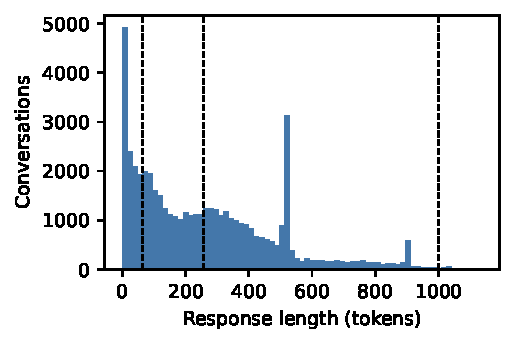
\includegraphics[width=0.9\linewidth]{length_hist.pdf}
\vspace{-0.6em}
\caption{Response lengths in the 50k subset. Dashed lines are bucket edges; the spike at 512 is a generation cap.}
\label{fig:hist}
\end{figure}

\section{Baseline}
The baselines need no learning. \textbf{FCFS} serves requests in arrival order and is the default in Orca and vLLM. \textbf{Shortest-prompt-first} serves the waiting request with the fewest prompt tokens, using prompt length as a free proxy for response length. \textbf{Oracle SJF} orders by true service time and is the upper bound. On the prediction side the baselines are the majority bucket and a logistic regression on log prompt length alone.

All policies run in the same simulator (\texttt{src/simulator.py}): one non-preemptive server, Poisson arrivals, and service time $s_i = a\,p_i + b\,o_i$ for $p_i$ prompt and $o_i$ output tokens, with $a = 0.5$\,ms and $b = 20$\,ms. When the server frees up it takes the waiting request with the smallest priority key, with ties going to the earlier arrival. The simulator reproduces the proposal's worked example (jobs of 20, 800, 50, 300 tokens arriving together give mean latency 720 under FCFS and 407.5 under SJF). Baseline results are in Tables~\ref{tab:pred} and~\ref{tab:sched}. Shortest-prompt-first is \emph{worse} than FCFS at every load, because prompt length carries almost no ordering signal here ($\tau = 0.008$).

\section{Main Approach}
\textbf{Model.} A prompt $x$ is mapped to features $\phi(x)$: 14 handcrafted values (log prompt tokens, log characters, line and question-mark counts, whether the first word is a long-form verb such as \emph{write} or \emph{explain} or a short-answer opener such as \emph{is} or \emph{what}, an explicit length request such as ``500 words'' and its size, brevity and detail cues, code markers, essay and list cues, and one-word-answer cues) plus TF-IDF unigrams and bigrams over the first 50 words (20k features). A classifier outputs $P(k \mid x)$ over the four buckets $k \in \{0,1,2,3\}$. We train a class-weighted multinomial logistic regression (LR) and a class-weighted gradient-boosted tree ensemble (GBM, LightGBM, 400 trees), choosing $C$ and the number of leaves by validation $\tau$.

\textbf{Ranking score.} The bucket alone gives only four priority levels, so the queue key is the expected bucket index
\[ r(x) = \textstyle\sum_{k=0}^{3} k \, P(k \mid x), \]
which is continuous and orders requests within a predicted bucket.

\textbf{Algorithm.} Predicted SJF is a priority queue on $r$: each arriving request is scored once and inserted; the server pops the smallest $r$.

\textbf{Example.} Take three unseen test prompts waiting together: (A) ``rustlang example using Arc and threads with anyhow to handle errors'' (true length 512), (B) ``create a dockerfile that changes the user to non-root'' (161), and (C) ``how am i?'' (55). All are short prompts (13, 12, and 4 tokens), so shortest-prompt-first cannot separate A from B. For B, $\phi$ fires the long-form-verb feature on \emph{create} alongside the TF-IDF terms; the GBM gives $r = 1.68$. A scores $1.89$ and C scores $0.66$. The queue serves C, B, A, which is the oracle order. With $b = 20$\,ms this gives a mean latency of about 6.7\,s against 12.8\,s for the arrival order A, B, C.

\section{Evaluation Metric}
\textbf{Prediction.} Four-class accuracy; macro-F1 $= \frac14\sum_k \frac{2 P_k R_k}{P_k + R_k}$ over per-bucket precision and recall, so the rare bucket counts equally; and Kendall's $\tau_b$ between $r(x_i)$ and true length $o_i$, i.e.\ concordant minus discordant pairs over all pairs, corrected for ties. $\tau$ is the main metric because SJF depends only on order.

\textbf{Scheduling.} With arrival $a_i$ and completion $c_i$, latency is $L_i = c_i - a_i$. We report mean latency, p99 latency, and
\[ \text{gap closed} = \frac{\bar L_{\text{FCFS}} - \bar L_{\text{policy}}}{\bar L_{\text{FCFS}} - \bar L_{\text{oracle}}}, \]
which is 0 for FCFS and 1 for oracle SJF. The 5k test prompts are replayed at loads $\rho = \lambda\,\mathbb{E}[s] \in \{0.5, 0.8, 0.95\}$ with five arrival seeds each. Qualitatively, we inspect the confusion matrix, the most important features, and which requests are starved.

\section{Results \& Analysis}
\label{sec:results}

\begin{table}[t]
\centering\small
\setlength{\tabcolsep}{4pt}
\begin{tabular}{lcccc}
\toprule
Model & Acc. & Macro-F1 & $\tau$ & $\tau$ (unseen) \\
\midrule
Majority bucket & 0.438 & 0.152 & 0 & 0 \\
Prompt length LR & 0.140 & 0.111 & 0.008 & $-0.014$ \\
LR, all features & 0.618 & 0.503 & 0.592 & 0.546 \\
GBM, all features & \textbf{0.700} & \textbf{0.528} & \textbf{0.619} & \textbf{0.571} \\
\bottomrule
\end{tabular}
\vspace{-0.4em}
\caption{Prediction on the 5k test set. ``Unseen'' excludes the 13.7\% of test prompts that occur verbatim in train.}
\label{tab:pred}
\end{table}

\begin{table}[t]
\centering\small
\setlength{\tabcolsep}{3pt}
\begin{tabular}{llrrr}
\toprule
$\rho$ & Policy & Mean (s) & p99 (s) & Gap closed \\
\midrule
0.5 & FCFS & 9.7 & 40.5 & 0 \\
 & Shortest prompt & 9.8 & 51.8 & $-0.04$ \\
 & Predicted SJF (LR) & 8.8 & 42.6 & 0.77 \\
 & Predicted SJF (GBM) & 8.8 & 43.2 & 0.80 \\
 & Oracle SJF & 8.6 & 39.8 & 1 \\
\midrule
0.8 & FCFS & 23.9 & 113.3 & 0 \\
 & Shortest prompt & 25.1 & 296.2 & $-0.13$ \\
 & Predicted SJF (LR) & 17.4 & 176.5 & 0.74 \\
 & Predicted SJF (GBM) & 16.9 & 163.9 & 0.80 \\
 & Oracle SJF & 15.1 & 131.7 & 1 \\
\midrule
0.95 & FCFS & 79.3 & 264.8 & 0 \\
 & Shortest prompt & 83.6 & 1359.4 & $-0.10$ \\
 & Predicted SJF (LR) & 46.6 & 912.0 & 0.71 \\
 & Predicted SJF (GBM) & 45.8 & 911.6 & 0.73 \\
 & Oracle SJF & 33.3 & 574.0 & 1 \\
\bottomrule
\end{tabular}
\vspace{-0.4em}
\caption{Scheduling results, averaged over five arrival seeds. Gap-closed standard deviation across seeds is at most 0.04 for the learned policies.}
\label{tab:sched}
\end{table}

\textbf{Prediction.} Table~\ref{tab:pred} shows that prompt length alone is useless as a ranker, while the full feature set reaches $\tau = 0.62$ (GBM) and $0.59$ (LR). The prompt-length LR falls below the majority baseline in accuracy because class weighting pushes a one-feature model toward the rare bucket. On unseen prompts $\tau$ drops by about 0.05, so roughly that much of the headline number comes from repeated prompts. The most important GBM features by gain are prompt size, question-mark count, the requested word count, and terms such as \emph{write}, \emph{answer}, and \emph{article about}.

The $>$1k bucket is not learnable at this scale: the test set has 15 such responses and the GBM recalls none (Figure~\ref{fig:cm}); class-weighted LR recalls 7 but mislabels 522 shorter responses as $>$1k. Most remaining error is between adjacent buckets, which costs little in ordering terms.

\textbf{Scheduling.} Table~\ref{tab:sched} shows predicted SJF with the GBM closing 80\%, 80\%, and 73\% of the FCFS-to-oracle gap in mean latency, cutting the mean from 79.3\,s to 45.8\,s at $\rho = 0.95$. As a reference, SJF on the \emph{true} bucket with FCFS inside each bucket closes 80\%, 74\%, and 72\%. The learned score matches a perfect four-bucket classifier because $r(x)$ is continuous and orders within buckets, which confirms that rank, not bucket accuracy, is the quantity to optimize.

The cost is the tail. At $\rho = 0.95$, p99 latency is 265\,s under FCFS, 574\,s under oracle SJF, and 912\,s under predicted SJF. Oracle SJF starves only requests that really are long; predicted SJF also starves short requests that were scored as long, and they wait behind everything else. The mean latency of the longest 10\% of jobs rises from 89\,s (FCFS) to 160\,s (GBM). Figure~\ref{fig:gap} also shows the gap closed falling as load rises, since longer queues give each ranking error more requests to affect.

\textbf{Label noise.} Among the 1{,}844 prompts that occur more than once in the 50k, only 71\% have all copies in a single bucket, and the median coefficient of variation of their lengths is 0.20. Repeated prompts are skewed toward templated inputs, so this is a rough estimate, but it shows that no prompt-only predictor can reach $\tau = 1$.

\textbf{Implications.} (1) The current buckets fit this data poorly: one is nearly empty and one holds 45\% of responses and 79\% of output tokens. Quantile buckets or a direct ranking loss should help. (2) Mean latency is already near what four buckets allow, so the remaining gain is in within-bucket order and in the tail. (3) The p99 blow-up makes the starvation-aware objective from the proposal necessary, not optional.

\begin{figure}[t]
\centering
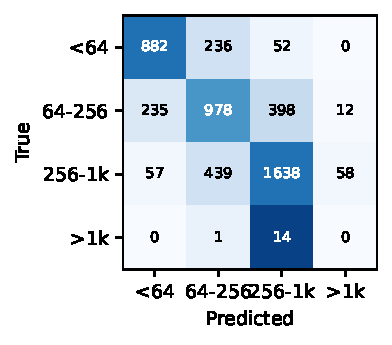
\includegraphics[width=0.62\linewidth]{confusion_gbm.pdf}
\vspace{-0.6em}
\caption{GBM confusion matrix on the test set (counts; shading is row-normalized).}
\label{fig:cm}
\end{figure}

\begin{figure}[t]
\centering
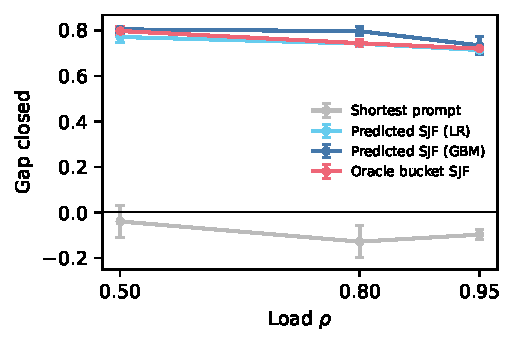
\includegraphics[width=0.85\linewidth]{gap_closed.pdf}
\vspace{-0.6em}
\caption{Fraction of the FCFS-to-oracle mean-latency gap closed, by load. Error bars are one standard deviation over five seeds.}
\label{fig:gap}
\end{figure}

\section{Code}
\url{https://github.com/YogeshSeeni/cs221-llm-length-prediction}

\section{Future Work}
(1) Fine-tune DistilBERT with an ordinal or pairwise RankNet loss and compare $\tau$, inference cost, and gap closed against the GBM. (2) Implement local search over adjacent swaps on $J(\pi) = \sum_i \hat C_i + \lambda \sum_i \max(0, \hat W_i - W_{\max})^2$, starting from predicted SJF, and sweep $\lambda$ to trace mean against p99 latency. (3) Replace the fixed buckets with quantile buckets, and split by prompt text to remove train/test overlap. (4) Because the 512-token cap removes the heavy tail that makes SJF most valuable, rerun the simulation with a synthetic heavy-tailed length distribution or regenerated uncapped responses. (5) Beyond ordering, an accurate length estimate would also allow KV-cache reservation, length-aware batching, admission control under overload, and routing long requests to separate replicas; we will evaluate at least memory reservation in the simulator if time allows.

\section{AI-Use Disclosure Statement}
% DRAFT: put this section in your own words before submitting.
I used Claude (Anthropic) at this stage for ideation and literature search only. For ideation, I used it to discuss the feedback on my proposal, namely how heavy-tailed response lengths could affect the project and what an accurate length prediction would enable beyond queue ordering, and to discuss how to organize prior systems in the literature review. For literature, I asked it to search for related work on response-length prediction and LLM request scheduling; it returned candidate papers with short summaries. I read the abstracts and relevant sections of the papers I cite, checked the figures I quote against the papers, and chose which to cite.

I did not use generative AI to write any text in this report, to implement any code (dataset construction, features, models, baselines, simulator, evaluation, or figures), to collect or label data, to run experiments, or to analyze results. I take full responsibility for the contents of this report.

\bibliographystyle{unsrtnat}
\bibliography{references}
\end{document}
